%%%%%%%%%%%%%%%%%%%%%%%%%%%%%%%%%%%%%%%%%
% Beamer Presentation
% LaTeX Template
% Version 1.0 (10/11/12)
%
% This template has been downloaded from:
% http://www.LaTeXTemplates.com
%
% License:
% CC BY-NC-SA 3.0 (http://creativecommons.org/licenses/by-nc-sa/3.0/)
%
%%%%%%%%%%%%%%%%%%%%%%%%%%%%%%%%%%%%%%%%%

%----------------------------------------------------------------------------------------
%	PACKAGES AND THEMES
%----------------------------------------------------------------------------------------

\documentclass{beamer}

\mode<presentation> {

% The Beamer class comes with a number of default slide themes
% which change the colors and layouts of slides. Below this is a list
% of all the themes, uncomment each in turn to see what they look like.

%\usetheme{default}
%\usetheme{AnnArbor}
%\usetheme{Antibes}
%\usetheme{Bergen}
%\usetheme{Berkeley}
%\usetheme{Berlin}
%\usetheme{Boadilla}
%\usetheme{CambridgeUS}
%\usetheme{Copenhagen}
%\usetheme{Darmstadt}
%\usetheme{Dresden}
%\usetheme{Frankfurt}
%\usetheme{Goettingen}
%\usetheme{Hannover}
%\usetheme{Ilmenau}
%\usetheme{JuanLesPins}
%\usetheme{Luebeck}
\usetheme{Madrid}
%\usetheme{Malmoe}
%\usetheme{Marburg}
%\usetheme{Montpellier}
%\usetheme{PaloAlto}
%\usetheme{Pittsburgh}
%\usetheme{Rochester}
%\usetheme{Singapore}
%\usetheme{Szeged}
%\usetheme{Warsaw}

% As well as themes, the Beamer class has a number of color themes
% for any slide theme. Uncomment each of these in turn to see how it
% changes the colors of your current slide theme.

%\usecolortheme{albatross}
%\usecolortheme{beaver}
%\usecolortheme{beetle}
%\usecolortheme{crane}
%\usecolortheme{dolphin}
%\usecolortheme{dove}
%\usecolortheme{fly}
%\usecolortheme{lily}
%\usecolortheme{orchid}
%\usecolortheme{rose}
%\usecolortheme{seagull}
%\usecolortheme{seahorse}
%\usecolortheme{whale}
%\usecolortheme{wolverine}

%\setbeamertemplate{footline} % To remove the footer line in all slides uncomment this line
%\setbeamertemplate{footline}[page number] % To replace the footer line in all slides with a simple slide count uncomment this line

%\setbeamertemplate{navigation symbols}{} % To remove the navigation symbols from the bottom of all slides uncomment this line
}

\usepackage{graphicx} % Allows including images
\usepackage{booktabs} % Allows the use of \toprule, \midrule and \bottomrule in tables
\usepackage{listings}
\usepackage{amsmath}
\usepackage{algpseudocode,algorithm,algorithmicx}

\lstdefinestyle{customjava}{
  breaklines=true,
  frame=L,
  xleftmargin=\parindent,
  language=Java,
  showstringspaces=false,
  basicstyle=\footnotesize\ttfamily,
  keywordstyle=\bfseries\color{green!40!black},
  commentstyle=\itshape\color{gray!40!black},
  identifierstyle=\color{blue},
  stringstyle=\color{orange},
}

\lstdefinestyle{customcpp}{
  breaklines=true,
  frame=L,
  xleftmargin=\parindent,
  language=C++,
  showstringspaces=false,
  basicstyle=\footnotesize\ttfamily,
  keywordstyle=\bfseries\color{green!40!black},
  commentstyle=\itshape\color{gray!40!black},
  identifierstyle=\color{blue},
  stringstyle=\color{orange},
}
%----------------------------------------------------------------------------------------
%	TITLE PAGE
%----------------------------------------------------------------------------------------

\title[Interprocess Communication]{Interprocess Communication} % The short title appears at the bottom of every slide, the full title is only on the title page

\author{Jonathan Windle} % Your name
\institute[UEA] % Your institution as it will appear on the bottom of every slide, may be shorthand to save space
{
University of East Anglia \\ % Your institution for the title page
\medskip
\textit{J.Windle@uea.ac.uk} % Your email address
}
\date{\today} % Date, can be changed to a custom date

\begin{document}

\begin{frame}
\titlepage % Print the title page as the first slide
\end{frame}

\begin{frame}[allowframebreaks]
\frametitle{Overview} % Table of contents slide, comment this block out to remove it
\tableofcontents % Throughout your presentation, if you choose to use \section{} and \subsection{} commands, these will automatically be printed on this slide as an overview of your presentation
\end{frame}

%-------------------------------------------------------------------
\section{Terminology}
\begin{frame}
\frametitle{Terminology}
\begin{itemize}
\item \textbf{Memory:} Numerically addressable data storage
\item \textbf{Address:} Number used to identify a memory location
\item \textbf{Segment:} A contiguous block of memory
\item \textbf{Address space:} Range of addresses used by a process
\item \textbf{Memory image:} Contents of an address space
\item \textbf{Primary memory:} Main memory
\item \textbf{Secondary memory:} Disk storage
\end{itemize}
\end{frame}
%--------------------------------------------------------------------
\section{Requirements}
\begin{frame}
\frametitle{Requirements}
\begin{itemize}
\item OS Memory manager must provide:
\begin{itemize}
\item Ability to relocate a process in memory
\item Protection of memory belonging to a process
\item Ability to share memory between processes
\item Logical and efficient organisation of memory
\item Physical organisation of memory
\end{itemize}
\item Programmers ideally like:
\begin{itemize}
\item Unlimited amount of memory
\item Super-fast read-write access times
\end{itemize}
\item In reality they get a range of memory systems, each having:
\begin{itemize}
\item Different capacities
\item Different access time
\item Different cost per bit
\end{itemize}
\item Although size of main memory is increasing, the faster programmers fill it.
\end{itemize}
\end{frame}
%-------------------------------------------------------------------
\section{Memory Hierarchy}
\begin{frame}
\frametitle{Memory Hierarchy}
\begin{itemize}
\item General Rule:
\begin{itemize}
\item Faster memory access times cost more
\item Computers are designed to provide:
\begin{itemize}
\item Large capacity of (cheap) slow memory
\item Smaller capacities of (expensive) fast memory
\end{itemize}
\item OS must decide what data gets stored where
\item Optimise overall performance
\end{itemize}
\end{itemize}
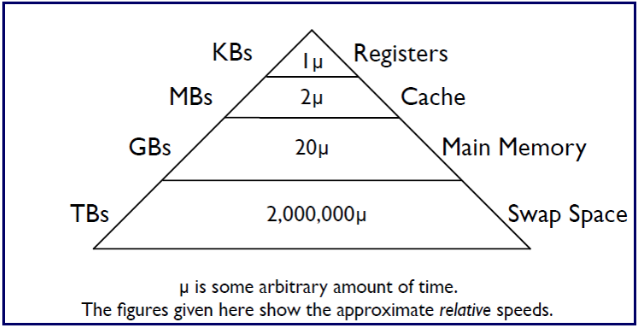
\includegraphics[scale=0.35]{hier.png}
\end{frame}
%------------------------------------------------------------------
\subsection{Memory Usage}
\begin{frame}
\frametitle{Memory Usage}
\begin{itemize}
\item Initially proceeses are loaded into secondary memory
\item Some, or all of data is then copied into main memory
\item Frequently used data can be copied into cache
\item When processes run, variables are copied into CPU registers
\item We potentially have up to four copies of the data
\begin{itemize}
\item We COPY rather than MOVE data since only need to MOVE when updates occur.
\end{itemize}
\end{itemize}
\end{frame}
%----------------------------------------------------------------
\subsection{Memory Binding}
\begin{frame}
\frametitle{Memory Binding}
\begin{itemize}
\item Source code is written in the form of text
\item The source code indirectly defines the instructions to execute
\item The variables define placeholders for data to act upon
\item Instructions are usually executed in sequential fashion, but there are often branches to different locations
\item For example, sub-routine calls, \texttt{switch} statements, \texttt{for} loops etc.
\end{itemize}
\end{frame}
%-----------------------------------------------------------------
\section{Memory Management}
\subsection{Uniprogramming Memory Management}
\begin{frame}
\frametitle{Uniprogramming Memory Management}
\begin{itemize}
\item Only one process can be run at a time
\item Process is loaded into memory and runs
\item No real need for memory management
\begin{itemize}
\item Process has access to whole of main user memory
\item Virtual memory == physical memory
\end{itemize}
\item Programs loaded to the first location in user memory
\item Location referred to as the base address
\item References to variables are offsets from base address.
\end{itemize}
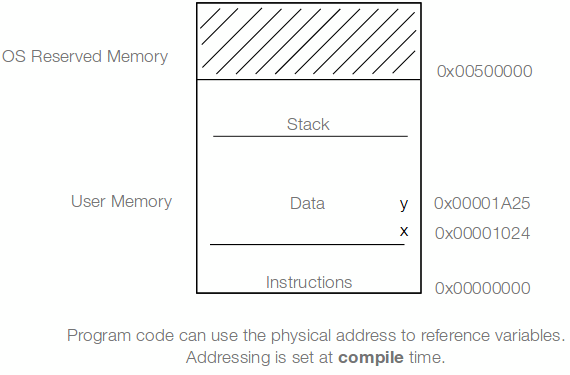
\includegraphics[scale=0.3]{uni.png}
\end{frame}
%------------------------------------------------------------------
\subsection{Multiprogramming Memory Addressing}
\begin{frame}
\frametitle{Multiprogramming Memory Addressing}
\begin{itemize}
\item Addressing is more tricky if there are many processes in memory
\item Processes cannot share the same physical location
\item Divide memory into number of segments:
\begin{itemize}
\item Segment sizes could be fixed/variable or unequal/equal
\end{itemize}
\item Processes must know where their variable are stored:
\begin{itemize}
\item This is not known at compile time
\item Generally memory references are still relative to a base address
\item Proceses cannot share same physical locations
\end{itemize}
\item Memory address used at compile time is virtual.
\end{itemize}
\end{frame}
%--------------------------------------------------------------------
\section{Static Translation}
\begin{frame}
\frametitle{Static Translation}
\begin{itemize}
\item All programs assume base location of 0.
\item {\color{red}Relocation loader} adjusts memory references to reflect actual base location when process is loaded:
\begin{itemize}
\item Offset relative to (compile time) base address (i.e. 0).
\item Relocation is performed when program is loaded.
\item Linker (compilation stage) lists which references need relocation
\item References are corrected when the program is loaded.
\item References are corrected when program is loaded.
\end{itemize}
\item Physical memory references set at LOAD time.
\end{itemize}
\end{frame}
%------------------------------------------------------------------
\subsection{Problems}
\begin{frame}
\frametitle{Problems}
\begin{itemize}
\item Simple relocation strategy is Static:
\begin{itemize}
\item Difficult to recover fragmented memory
\end{itemize}
\item Processes cannot be moved into physical memory
\item No mechanism for sharing memory
\item There is no memory protection between processes
\item Assumes memory requirements are known and fixed.
\end{itemize}
\end{frame}
%-------------------------------------------------------------------
\section{Dynamic Translation}
\begin{frame}
\frametitle{Dynamic Translation}
\begin{itemize}
\item Add base register to store segment base address
\item Use the contents of this register to offset address references within the program
\item In this way, addresses used by the CPU are virtual.
\item Base register translates memory addresses.
\item Translation is transparent to the process/CPU
\item Physical addresses are set at run time
\item Base + offset is computed for every read/write operation
\item Offset computed by hardware
\item Need a record of base address for each process.
\item Cannot have a dedicated (Base) register for each process
\item Instead the address is stores in the Process Control Block (PCB).
\end{itemize}
\end{frame}
%----------------------------------------------------------------------
\subsection{Alternate...}
\begin{frame}
\frametitle{Alternate...}
\begin{itemize}
\item To allow processses to be relocated in memory while running, the {\color{red}base register} can store the base address of the current segment for the process.
\item The contents of this register are then often used to offset memory references within the program
\item The CPU is utilising a {\color{green}virtual address}:
\begin{itemize}
\item It does not use the address of physical location in memory
\item Thus, the base register translates virtual addresses to physical addresses
\end{itemize}
\item The translation is transparent to process/CPU
\item Addressing is set at run time.
\item Memory references must be offset for every read/write operation, this must be quick and so it is done in hardware
\item Every process has a different base address, but there cannot be a dedicated base register for each
\item Instead the base address is stored in the Process Control Block (PCB).
\end{itemize}
\end{frame}
%------------------------------------------------------------------
\subsection{Diagram}
\begin{frame}
\frametitle{Diagram}
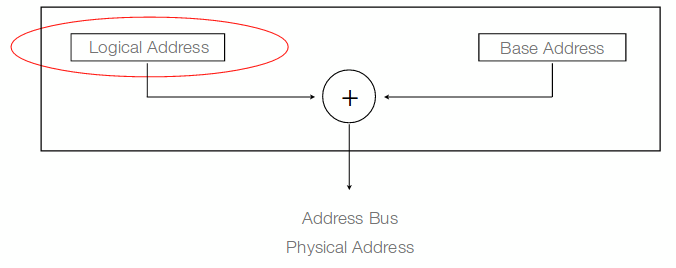
\includegraphics[scale=0.5]{dynam.png}
\end{frame}
%-------------------------------------------------------------------
\section{Memory Segmentation}
\subsection{Fixed and Equal-Sized Memory Segments}
\begin{frame}
\frametitle{Fixed and Equal-Sized Memory Segments}
\begin{itemize}
\item Equal segment sizes are wasteful
\item Small processes are likely to fill a segment
\item If segment size is large, lots of memory unused
\item Only one process may occupy a segment
\end{itemize}
\end{frame}
%-------------------------------------------------------------------
\subsection{Fixed and Unequal-sized Memory Segments}
\begin{frame}
\frametitle{Fixed and Unequal-sized Memory Segments}
\begin{itemize}
\item Create fixed-sized segments of differing size
\item Assign processes to ones of best fit
\item As a process completes, load next in the queue.
\end{itemize}
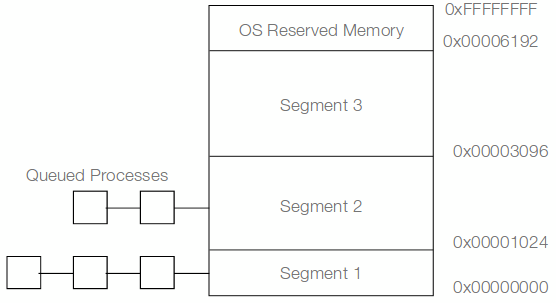
\includegraphics[scale=0.35]{uneq.png}
\end{frame}
%-------------------------------------------------------------------
\subsection{Limitations}
\begin{frame}
\frametitle{Limitations}
\begin{itemize}
\item Fixed segment sizes leads to internal fragmentation, assumes fixed memory requirements for all processes
\item Doesn't allow for more physical memory than is available
\item Queued processes must wait for an appropriate sized segment
\item No mechanism for protecting memory
\end{itemize}
\end{frame}
%------------------------------------------------------------------
\section{Memory Protection}
\begin{frame}
\frametitle{Memory Protection}
\begin{itemize}
\item Simple approach uses another hardware register
\item Register is loaded with segment size
\item Logicl address is compared with contents of limit register
\item If outside the allowed range, generate exception (Seg fault).
\end{itemize}
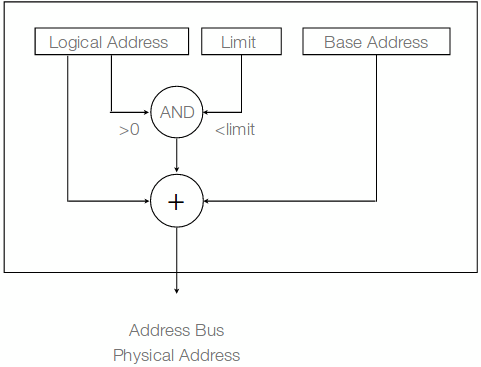
\includegraphics[scale=0.35]{lim.png}
\end{frame}
%------------------------------------------------------------------
\section{Allocating processes}
\begin{frame}
\frametitle{Allocating Processes}
\begin{itemize}
\item Must select a process to fit a segment:
\begin{itemize}
\item First-fit strategy
\item Best-fit strategy
\item Worst-fit strategy
\end{itemize}
\end{itemize}
\end{frame}
%-------------------------------------------------------------------
\section{Summary}
\begin{frame}
\frametitle{Summary}
\begin{itemize}
\item Memory comprises a range of technologies configured as a hierarchy
\item Memory divided into segments, running processees
\item CPU operates in virtual memory space which is mapped onto physical space
\item Programs need to be bound to memory:
\begin{itemize}
\item By the compiler
\item By the loader
\end{itemize}
\item Later supports relocation: efficient use of main memory
\end{itemize}
\end{frame}
%------------------------------------------------------------------

\begin{frame} 
\Huge{\centerline{The End}}
\end{frame}

\end{document}